\documentclass[10pt,twocolumn,letterpaper]{article}
%% Welcome to Overleaf!
%% If this is your first time using LaTeX, it might be worth going through this brief presentation:
%% https://www.overleaf.com/latex/learn/free-online-introduction-to-latex-part-1

%% Researchers have been using LaTeX for decades to typeset their papers, producing beautiful, crisp documents in the process. By learning LaTeX, you are effectively following in their footsteps, and learning a highly valuable skill!

%% The \usepackage commands below can be thought of as analogous to importing libraries into Python, for instance. We've pre-formatted this for you, so you can skip right ahead to the title below.

%% Language and font encodings
\usepackage[brazil]{babel}
\usepackage[utf8x]{inputenc}
\usepackage[T1]{fontenc}

%% Sets page size and margins
\usepackage[a4paper,top=3cm,bottom=2cm,left=3cm,right=2cm,marginparwidth=1.75cm]{geometry}

%% Useful packages
\usepackage{amsmath}
\usepackage{graphicx}
\usepackage[colorinlistoftodos]{todonotes}
\usepackage[colorlinks=true, allcolors=blue]{hyperref}
\usepackage[numbers]{natbib}
\bibliographystyle{IEEEtranN}
%% Title
\title{
		\usefont{OT1}{bch}{b}{n}
		\normalfont \normalsize \textsc{EEL7323-08235 Programação C++ para Sistemas Embarcados} \\ [10pt]
		\huge Bússola eletrônica de 2 eixos \\
}
\selectlanguage{english}
\usepackage{authblk}
\renewcommand\Authand{, e }
\renewcommand\Authands{, e }
\author[1]{Gustavo Batistell}
\affil[1]{UFSC - Universidade Federal de Santa Catarina \\
\newline Curso de Graduação em Engenharia Eletrônica}

\begin{document}
\maketitle

\section{Introdução}

O objetivo deste projeto é desenvolver um magnetômetro eletrônico capaz de apresentar, entregar e salvar os dados de \emph{heading}, 
ou direção em relação ao campo magnético terrestre, ou seja, a direção apontada pelo equipamento.
Os magnetômetros eletrônicos são parte importante na instrumentação de embarcações, aeronaves, submarinos, satélites, etc e durante 
a realização do estágio no Laboratório do Grupo Drakkar Atlantec em Florianópolis, foi constatada a demanda para dominar tanto o 
ajuste quanto a calibração deste tipo de instrumento. Apesar da empresa contar com as boninas de Helmhotz com controlador e um 
magnetômetro  de referência, tanto a parte eletrônica quanto os softwares embarcados carecem de atualização, melhoria e nova 
implementação para completo domínio do funcionamento. Essa necessidade de dominar (novamente) por completo o sistema surgiu devido 
perda de documentação e dos códigos originais com o passar dos anos. \\
Para isso, a tarefa do desenvolvimento inicial foi dividida em duas partes: uma parte para acionamento (driver) e outra parte para 
um magnetômetro, este último no qual fiquei incumbido.\\
Assim, utilizado um módulo micro-controlado ARM RP2040 Raspberry Pi Pico \cite{RP2040_Datasheet}, um módulo magnetômetro para medir 
o campo magnético em pelo menos 2 eixos (seja o HMC5883 ou HoneyWell HMC1002/2300 disponíveis no laboratório), realizar o acionamento 
de leds para apresentar o \emph{heading}, realizar log de dados e suportar acesso via UART/USB e Wireless. Ver diagrama da 
\autoref{fig:Diagrama_blocos}.

\begin{figure}[ht]
  \centering
  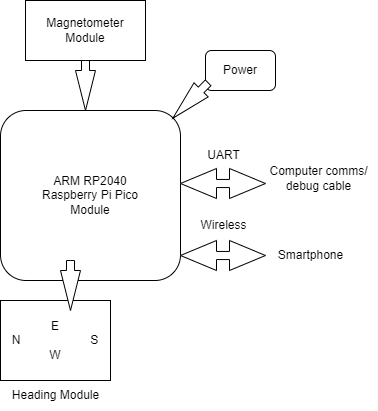
\includegraphics[width=\linewidth]{figures/ProjetoFinalCPP_Diagrama.png}
  \caption{Diagrama de blocos revisado do projeto.}
  \label{fig:Diagrama_blocos}
\end{figure}

\section{Requisitos}

Os requisitos de projeto foram combinados com a demanda do Laboratório do Grupo Drakkar Atlantec e as 
especificações solicitadas pelo professor, aproveitando-se da portabilidade e modularidade com a 
linguagem de programação C++ e os conceitos de orientação a objetos, polimorfismo, classes, etc. Assim, 
foram listados os requisitos de desenvolvimento combinados para uma Bússola Eletrônica conforme segue:

\begin{itemize}
    \item Apresente em mostrador simples de LEDs o \emph{heading} em 8 direções: N, NE, E, SE, S, SW, W e NW.
    \item Utilize um módulo de magnetômetro de pelo menos 2 eixos (seja analógico ou digital) para obtenção 
    das componentes de campo magnético.
    \item Com as componentes X e Y de campo magnético calcular a direção (em graus de 0 a 360) que também 
    pode ser utilizada para o \emph{heading}.
    \item Realizar log da ID, timeStamp e dados.
    \item Aceitar a consulta e envio deste log para um \emph{host}.
    \item Aceitar comunicação via UART/USB.
    \item Aceitar comunicação \emph{wireless}.
    \item O \emph{host} pode conferir a listagem do log.
    \item O \emph{host} pode conferir o tempo em que a Bússola Eletrônica se manteve ativa 
\end{itemize}


\section{Design Proposto}

Como o microcontrolador ARM RP2040 \cite{RP2040_Datasheet} é \emph{dual-core} foi decidido implementar 2 máquinas de estado. Uma 
delas para a aplicação da Bússola Eletrônica propriamente dita, que ao ser iniciada segue diretamente para o estado de aquisição 
de dados brutos, depois para um estado que calcula a direção a partir das componentes X e Y dos dados brutos, outro estado que 
armazena o log e finalmente um estado que exibe o \emph{heading}. Essa primeira máquina de estados na \emph{Trhead 1} é apresentada
na \autoref{fig:maquina_estados1} e é importante destacar a importância dela na gravação/escrita em RAM.
\begin{figure}[h]
  \centering
  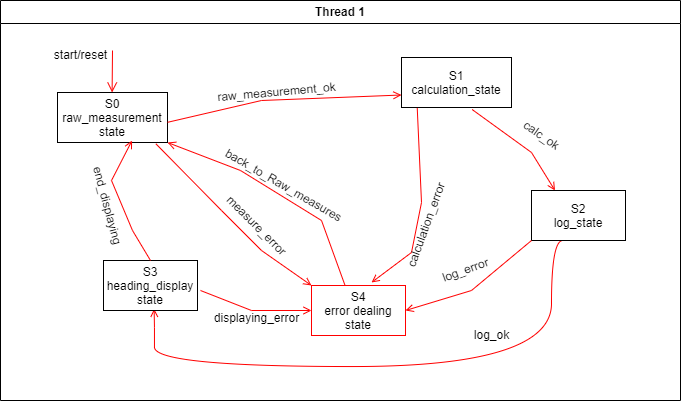
\includegraphics[width=\linewidth]{figures/maquina_estados1.png}
  \caption{Maquina de estados principal (com gravação em memória).}
  \label{fig:maquina_estados1}
\end{figure}
Já a segunda máquina de estados na \emph{Trhead 2} é incumbida de controlar a conectividade UART e \emph{Wireless}, conforme mostrado 
na a \autoref{fig:maquina_estados2}. Esta máquina de estados tem um estado de \emph{idle} para quando não houver conexão, um estado 
para conexão \emph{wireless} estabelecida, um estado para o wirelessRequest, um estado para quando a conexão UART é estabelecida, um 
estado para o UARTrequest e um estado para tratamento de erros. Esta máquina desta \emph{Trhead 2} apenas acessa os dados. Essa 
distinção entre gravação e acesso deste projeto em específico é importante para evitar problemas de leitura e escrita usuais em 
programação concorrente quando mais de uma \emph{trhead} é possível.
\begin{figure}[h]
  \centering
  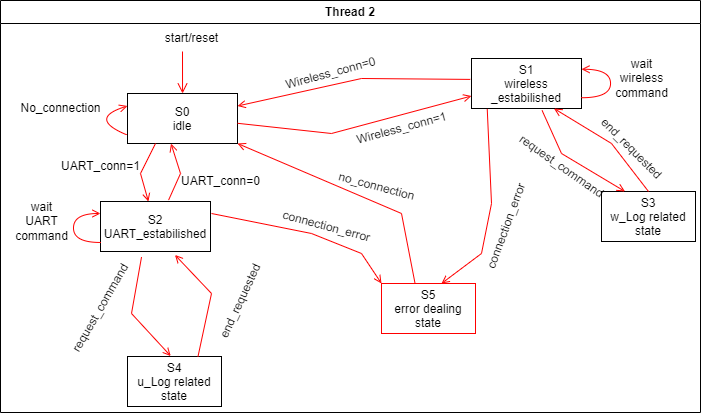
\includegraphics[width=\linewidth]{figures/maquina_estados2.2.png}
  \caption{Maquina de estados secundária para conexões UART e Wireless (apenas acesso a memória).}
  \label{fig:maquina_estados2}
\end{figure}

%\begin{figure}
%  \centering
%  \includegraphics[width=\linewidth]{figures/Tabela-de-estados.png}
%  \caption{Tabela de estados.}
%\end{figure}

Para garantir a modularidade do projeto, o diagrama de classes proposto utilizou de 5 níveis de abstração que são listados 
abaixo em uma abordagem "de dentro para fora":
\begin{itemize}
  \item Hardware Abstraction Layer (HAL): Responsável por abstrair o hardware subjacente, incluindo os módulos do SDK da Raspberry Pi Pico.
  \item Device Drivers Layer: Gerencia os drivers para GPIO, UART, comunicação sem fio e o magnetômetro.
  \item Processing Layer: Lida com o processamento dos dados, incluindo a classe `DirectionCalculator`. Esta camada também pode ser usada 
  para implementações futuras de técnicas de Digital Signal Processing como média móvel, dizimação, etc.
  \item Control/Application Layer: Responsável por controlar as partes funcionais do equipamento. É o ponto central onde as operações 
  funcionais são coordenadas. 
  \item User Interaction Layer: É a camada mais externa que lida com a interação do usuário, incluindo as classes `HeadingDisplay`, `Log`, 
  e as interfaces de comunicação com o usuário.
\end{itemize}
Essa organização se apresentou clara e permite uma separação adequada de responsabilidades em cada camada de classes do sistema, 
o que é uma boa prática para melhor documentar, estruturar e facilitar a compreensão e manutenção do projeto. O diagrama de classes 
pode ser visto na \autoref{fig:diagrama-classes} do Apêndice A.

%\section{Resultados}

%O software foi implementado e testado na plataforma Atlys e o comportamento do controlador funcionou conforme a especificação.
%Uma demonstração do funcionamento dos botões e terminal foi realizada em sala, simulando situações de inserção de moedas, obtenção de refrigerante e devolução do montante acumulado, e os logs resultantes podem ser vistos no \autoref{apendice-a}.
%A funcionalidade do display Oled não foi implementada em sala por uma questão de tempo, visto que a equipe já havia utilizado o diplay Oled em exercícios anteriores, então decidiu focar nas funcionalidades que ainda não haviam sido exploradas pela equipe.
%O código fonte encontra-se disponível no GitHub \cite{src-github}

%\section*{Conclusão}

%Com o desenvolvimento deste projeto, os benefícios do paradigma de programação orientada a objetos são evidentes.
%Por exemplo, a escolha de implementação da máquina de estados utilizando herança e polimorfismo, além de estar mais condizente com os assuntos abordados em aula, se provou mais organizada e de mais fácil manutenção quando comparada com a implementação mais comumente empregada em linguagem C, utilizando enums e switch/case.
%Esta abordagem facilita a implementação/inserção de novos estados, ou alterações nos estados já existentes.
%Outra vantagem é a modularidade do código. As classes Keyboard e Oled podem facilmente ser reutilizadas em outras aplicações que necessitem dessas funcionalidades.

\bibliography{bibliography}
\onecolumn
\appendix{Apêndice A}
\label{apendice-a}
%\section{Apêndice A}
\begin{figure}[h]
  \centering
  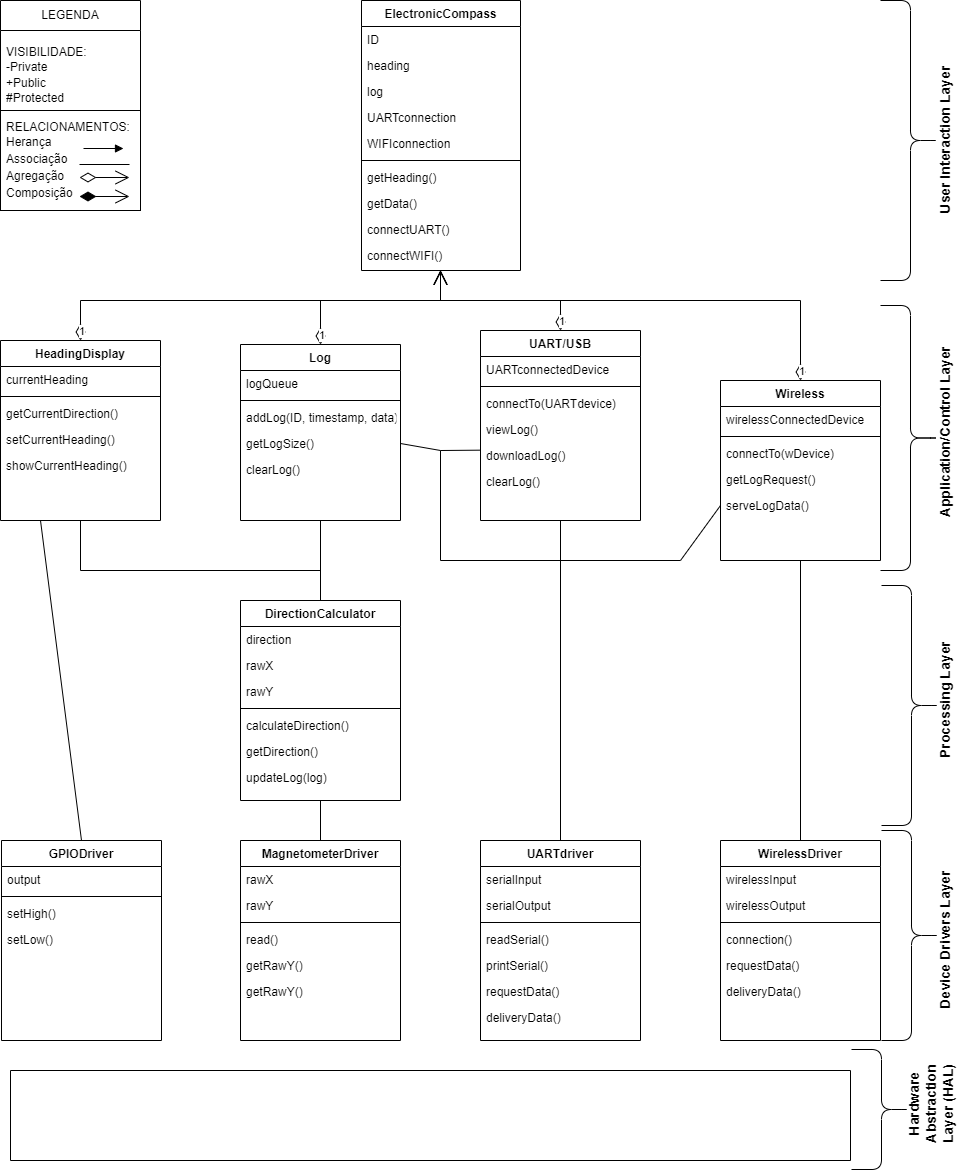
\includegraphics[keepaspectratio=true,scale=0.44]{figures/Diagrama_Classe_Projeto_Final.png}
  \caption{Diagrama de classes do projeto organizado em camadas.}
  \label{fig:diagrama-classes}
\end{figure}

%Logs gerados na demonstração em sala:
%{\scriptsize
%\begin{verbatim}
%grd...
%\end{verbatim}
%}
\onecolumn
\appendix{Apêndice B}
\label{apendice-b}

\subsection*{Plano de testes da Bússola eletrônica de 2 Eixos}
\begin{figure}[h]
  \centering
  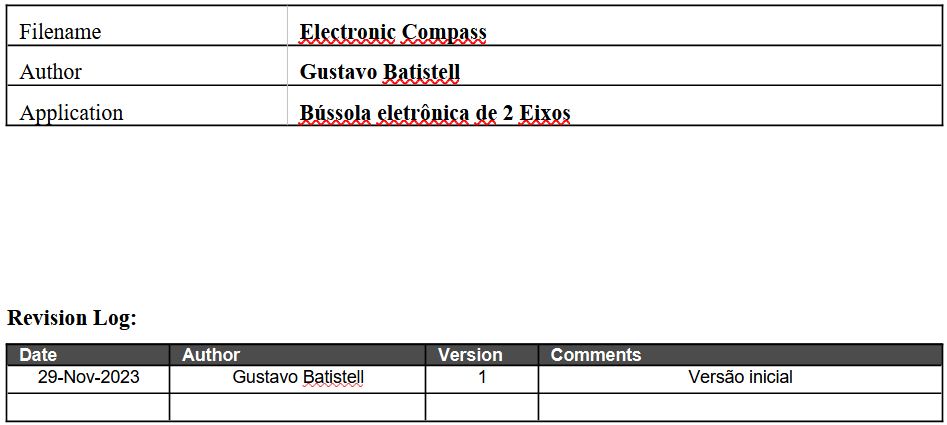
\includegraphics[keepaspectratio=true,scale=0.44]{figures/PlanoTestes.png}
 % \caption{Diagrama de classes do projeto organizado em camadas.}
  \label{fig:diagrama-classes}
\end{figure}

\subsection*{Introdução}
O objetivo desse plano de teste é orientar o teste de funcionamento do sistema Bússola Eletrônica	de 2 Eixos e suas partes.
\subsection*{Ambiente}
Uso de computador tipo PC rodando máquina virtual WSL Ubuntu no sistema operacional Windows 10 ou 11.
\subsection*{Processo}
\begin{itemize}
  \item Ligar o computador
  \item Rodar o WSL
  \item Clonar o repositório \cite{src-github} para a pasta local HOME.
  \item Entrar na pasta ~/ElectronicCompass\$ 
  \item Rodar a aplicação com o comando pcHost
\end{itemize}

\subsection*{Testes 1}
Resultados esperados:
\begin{itemize}
  \item Obter sucesso na conexão da comunicação
  \item Conseguir visualizar o tamanho do log de dados
  \item Visualizar os dados do período desejado
  \item Salvar os dados do período desejado
  \item Sair da aplicação com sucesso
\end{itemize}

\begin{itemize}
  \item Conferir exibição do menu de seleção na terminal
  \item Digitar a opção 1
  \item Verificar status da conexão
  \item Digitar a opção 2 para visualizar o tamanho do log de dados
  \item Digitar a opção 3 para visualizar os dados do log
  \item Digitar a opção 4 para salvar os dados do log
  \item Digitar a opção X para encerrar a aplicação
\end{itemize}

\end{document}
